
% Asset ID: A21RadiansTikZ-007
% Purpose: Show small angle approximations near zero, marked as boundary-risk support unless separately confirmed.
\documentclass[tikz,border=8pt]{standalone}
\usepackage{pgfplots}
\pgfplotsset{compat=1.18}
\begin{document}
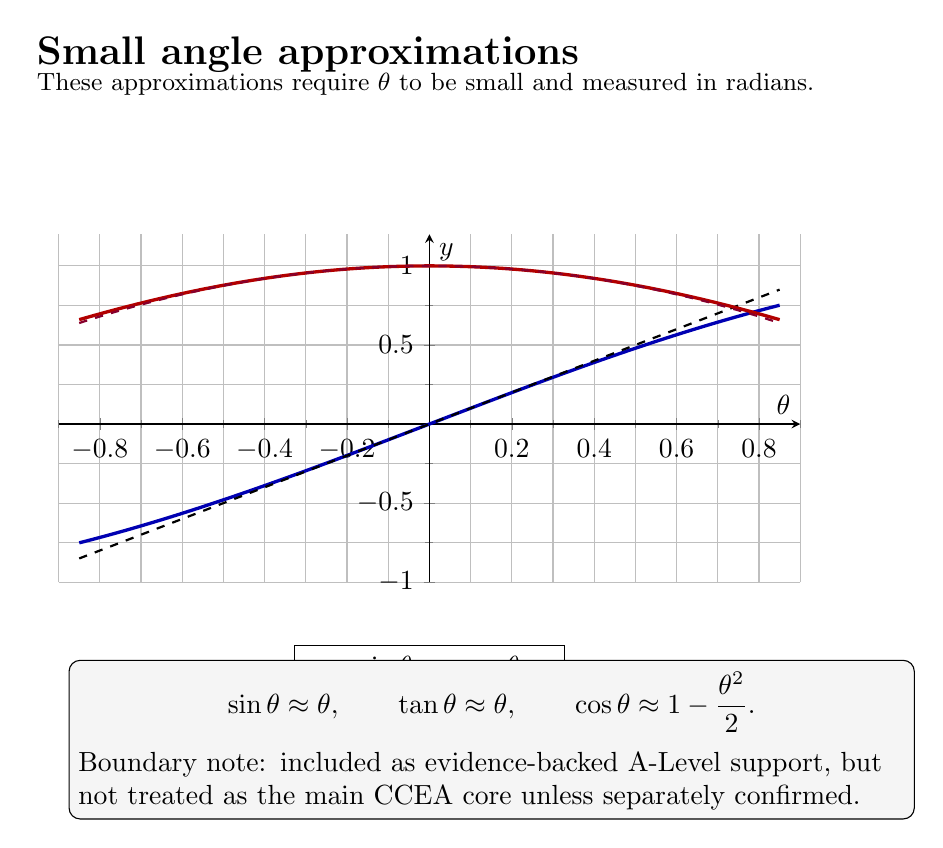
\begin{tikzpicture}
\node[anchor=west,font=\bfseries\Large] at (-0.4,6.7) {Small angle approximations};
\node[anchor=west,font=\small] at (-0.4,6.32) {These approximations require \(\theta\) to be small and measured in radians.};
\begin{axis}[width=11cm,height=6cm,axis lines=middle,xmin=-0.9,xmax=0.9,ymin=-1.0,ymax=1.2,xlabel={\(\theta\)},ylabel={\(y\)},samples=200,domain=-0.85:0.85,legend style={at={(0.5,-0.18)},anchor=north,legend columns=2},grid=both,minor tick num=1]
\addplot[very thick,blue!70!black] {sin(deg(x))};\addlegendentry{\(\sin\theta\)}
\addplot[thick,black,dashed] {x};\addlegendentry{\(\theta\)}
\addplot[very thick,red!70!black] {cos(deg(x))};\addlegendentry{\(\cos\theta\)}
\addplot[thick,purple!70!black,dashed] {1 - x^2/2};\addlegendentry{\(1-\frac{\theta^2}{2}\)}
\end{axis}
\node[draw,rounded corners,fill=gray!8,align=left,text width=10.5cm] at (5.5,-2.0) {\[\sin\theta\approx\theta,\qquad \tan\theta\approx\theta,\qquad \cos\theta\approx1-\frac{\theta^2}{2}.\] Boundary note: included as evidence-backed A-Level support, but not treated as the main CCEA core unless separately confirmed.};
\end{tikzpicture}
\end{document}
